\chapter{質量を持つ弱い交換、仮想粒子、そして破れた対称性}

標準模型の群は、フェルミオン表の上で許される運動の集合として読むと、はるかに謎めかなくなる。色変換は赤、緑、青の間を縦に動く。荷電弱変換はクォークとレプトンの二重項の中で横に動く。電磁位相変換は第三の操作を与える。対応するゲージボソンは、対称性が見つかった後に付け加えられた飾りではない。ゲージボソンを放出することは、対称性の生成子が記述するのと同じ状態変化を物理的に実行することである。

この観察が本講義の主要な問いを設定する。弱い頂点は電磁頂点と同程度の大きさの結合を持つが、ベータ崩壊は典型的な強い過程や電磁過程よりも桁違いに遅い。欠けている要素は伝播である。低運動量では、質量を持つ\(W\)を交換することは振幅に\(1/m_W^2\)程度の因子のコストを課す。まずこの主張を距離空間で展開し、次に運動量空間で展開し、実粒子と仮想粒子に関する長い議論を通してその帰結を追い、最後に自発的対称性の破れの最初の定性的模型に移る。

\section{フェルミオン表からゲージ対称性を読む}

\subsection{色は縦に作用する}

六つのクォークフレーバーを三つの弱い族に並べ、
\begin{equation}
  (u,d),\qquad(c,s),\qquad(t,b),
\end{equation}
各クォークに赤、緑、青の色ラベルを与える。得られるクォーク表は三つの色の行と六つのフレーバーの列を持つ。色\(SU(3)\)は任意の一つのフレーバー列の三つの項目を混合する。例えば、一つの生成子は赤いアップクォークを緑のアップクォークに変えうる。粒子の言葉では、同じ操作は補償する色と反色を運ぶグルーオンの放出を伴う。

同じ色変換はすべてのフレーバーに作用しなければならない。赤いアップクォークを緑のアップクォークに変えるグルーオンは、赤いトップクォークを緑のトップクォークに変えるグルーオンと同じ種類である。真の対称性操作は、第一世代に作用して他を無視するものではない。したがって色の運動は縦方向で普遍的である：
\begin{equation}
  q_r\longleftrightarrow q_g\longleftrightarrow q_b,
  \qquad q\in\{u,d,c,s,t,b\}.
\end{equation}
それは色を変えるがフレーバーは変えない。

これがゲージ群とそのゲージボソンの間の特徴的な関係である。無限小生成子は状態間の変換を記述し、対応するボソンの放出または吸収がそれらの変換を物理的過程として実現する。

\subsection{弱い変換は横に作用する}

荷電弱相互作用は反対の方向に動く。アップ型クォークは荷電弱ゲージボソンを放出して、色を変えずにそのダウン型パートナーになりうる：
\begin{equation}
  u_b\longrightarrow d_b+W^+.
\end{equation}
まったく同じ\(W^+\)が次でも起こる：
\begin{equation}
  c_g\longrightarrow s_g+W^+,
  \qquad
  t_r\longrightarrow b_r+W^+.
\end{equation}
ラベル\(r,g,b\)は傍観者である。グルーオンは表を横に動かず、荷電\(W\)ボソンは色を通って縦に動かない。

電磁位相対称性\(U(1)\)を加える。その下で荷電場はすべて位相を獲得する。第一近似の群構造は
\begin{equation}
  SU(3)\times SU(2)\times U(1).
\end{equation}
である。交差記号はこれらが独立な因子であることを意味する。一つは色に作用し、一つは弱い二重項に作用し、一つは位相によって作用する。これが有用な粗い描像であるが、まだ完全な電弱の話ではない。\editorialnote{正確な標準模型のゲージ群は慣例的に
\(SU(3)_c\times SU(2)_L\times U(1)_Y\)
と書かれる。弱い\(SU(2)_L\)は左手系二重項にのみ作用し、最終的な電磁\(U(1)_{\rm em}\)は対称性の破れの後に\(SU(2)_L\times U(1)_Y\)から現れる。本講義は、最後の二つの因子の第一近似の同定がまだ完全には整合していないことを明示的に警告している。後の講義が欠けているカイラル構造と電弱構造を与える。}

\subsection{同じパターンはレプトンを含む}

三つの色の行の下に無色のレプトンの行を置く：
\begin{equation}
\begin{array}{c|cc|cc|cc}
 &u&d&c&s&t&b\\ \hline
Q&+\frac23&-\frac13&+\frac23&-\frac13&+\frac23&-\frac13\\
\text{lepton partner}
 &\nu_e&e^-&\nu_\mu&\mu^-&\nu_\tau&\tau^-\\
Q&0&-1&0&-1&0&-1
\end{array}
\end{equation}
隣接する各対の中で電荷は一単位だけ異なる。それゆえ同じ荷電弱ゲージボソンが\(u\)を\(d\)に、\(c\)を\(s\)に、\(t\)を\(b\)に、そして荷電レプトンをそのニュートリノに結びつけうる。\(W\)頂点は適切な量子数と電荷差を気にするのであって、フェルミオンがクォークかレプトンかは気にしない。

\begin{figure}[htbp]
\centering
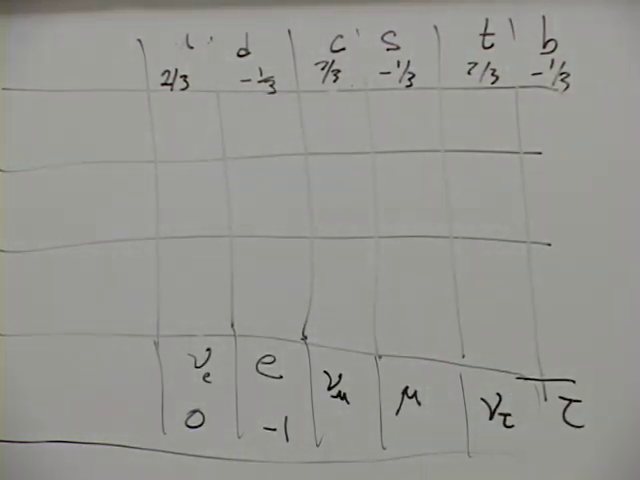
\includegraphics[width=0.88\textwidth]{lecture_06_figure_07.png}
\caption{完成したフェルミオン表：無色のレプトンの行の上に三つのクォーク色の行があり、クォークの電荷と三つのレプトン二重項が見える。}
\lectureframe{00:18:55}
\end{figure}

ミューオンは電子と同じ電荷と同じ既知の内部量子数を持つが、約二百倍重い。タウはさらに重い。ニュートリノの質量は非常に小さく、講義の議論では詳細には知られていなかった。観測された族の質量のパターンを説明する原理は、ここではまだ現れていない。

\begin{classroomqa}
\audiencequestion{なぜレプトン、バリオン、中間子はそのように呼ばれるのか？
\lecturetimestamp{00:19:02}}
\lecturerresponse{歴史的なギリシャ語の語根は、およそ軽い、重い、中間という意味であった。この質量に基づく命名は誤解を招くようになった。ミューオンはかつて、その質量が電子と陽子の質量の間にあることからミュ中間子と呼ばれたが、その相互作用は、それがパイオンよりもはるかに電子に似たレプトンであることを示している。今日、中間子とはクォーク--反クォークのハドロンを意味し、ボソンである。ミューオンは中間子ではない。}
\end{classroomqa}

\section{弱さの謎}

\subsection{具体的な荷電カレント過程}

中性子ベータ崩壊を作業図として用いる。価クォークの組成は
\begin{equation}
  n=udd,\qquad p=uud.
\end{equation}
である。1つのダウンクォークが遷移
\begin{equation}
  d\longrightarrow u+W^-,
\end{equation}
を起こし、荷電ボソンが
\begin{equation}
  W^-\longrightarrow e^-+\bar\nu_e.
\end{equation}
を生成する。合わせると、
\begin{equation}
  n\longrightarrow p+e^-+\bar\nu_e.
\end{equation}
となる。他の2つの価クォークはスペクテーターとしてそのまま持ち越される。第1の頂点で中性子は陽子になり、第2の頂点で、レプトン二重項を結ぶ同じ弱い相互作用が\(W^-\)を観測される電子と電子反ニュートリノに変換する。

\subsection{3つの結合、3つの大きく異なる印象}

QEDでは電子電荷\(e\)が頂点振幅である。これを二乗すると特徴的な放出確率が得られ、慣例的な因子は自然単位で
\begin{equation}
  \alpha=\frac{e^2}{4\pi}\simeq\frac1{137}
\end{equation}
にまとめられる。強い相互作用には結合定数\(g_s\)があり、典型的なハドロン的スケールではその類似物\(\alpha_s\)は\(0.2\)の程度でありうる。これは\(1/137\)よりはるかに大きいので、クォークが叩かれるとグルーオン放出は頻繁に起こる。

電荷をもつ弱い結合定数を\(g_w\)としよう。その二乗は途方もなく小さいわけではなく、ここで用いる桁程度のレベルでは電磁結合定数に匹敵する。それでも自由中性子は崩壊するまでにおよそ十五分待ち、一方強い崩壊はハドロンの通過時間程度で起こりうる。講義での歴史的見積もりは十二分という古い粗い数値を用いているが、どちらの数値でも同じ難問は避けられない。\editorialnote{現代の自由中性子の平均寿命はおよそ\(8.8\times10^2\,{\rm s}\)であり、主要な測定法の間には現在も実験的な緊張がある。講義の粗い寿命は精密値としてではなく、教育的なスケールとして保持されている。}
\begin{quote}
\(g_w\)が異常に小さくないのなら、何が弱い過程を弱くするのか。
\end{quote}

答えは頂点だけにあることはできない。すべてのファインマン図には伝播関数も含まれており、それは1つの頂点から別の頂点への中間的な運動を記述する因子である。

\section{距離空間における質量のある伝播関数}

\subsection{頂点だけが図のすべてではない}

ベータ崩壊の図には2つの弱い頂点があり、\(g_w\)の2つの冪と、それらを結ぶ\(W\)線に寄与する。位置空間の伝播関数を\(\Delta(x-y)\)で表す。ここで\(x\)は放出事象、\(y\)は吸収または変換事象である。それは、それら事象の間で場の擾乱を運ぶことに関連する振幅核である。

厳密な相対論的伝播関数は、我々が必要とする以上の構造を含んでいる。その重要な定性的特徴は質量への依存性である。短い空間的距離では、それは模式的には
\begin{equation}
  \Delta(d)\sim\frac1{d^2}.
\end{equation}
という冪的特異性をもつ。質量のない場は冪的な裾を保つ。対照的に、質量のある場は、間隔がそのコンプトンスケールに比べて大きくなると指数関数的に抑制される。したがってグラフは急激に下向きに曲がる。

\subsection{自然単位が曲がりを位置づける}


\begin{equation}
  c=\hbar=1.
\end{equation}
と置く。すると
\begin{equation}
  [m]=[E]=[p]=L^{-1}.
\end{equation}
となる。おなじみの関係が各等式を説明する。\(E=mc^2\)は質量とエネルギーを同一視し、一方\(p\,x\)は\(\hbar\)の次元をもつので、運動量と距離は逆の単位をもつ。したがって質量\(m\)から作ることのできる唯一の長さは
\begin{equation}
  d_m\sim\frac1m.
\end{equation}
である。定数を復元すると
\begin{equation}
  d_m\sim\frac{\hbar}{mc},
\end{equation}
となり、これはコンプトン波長である。より重い交換粒子はより短い有効到達距離をもつ。

\begin{figure}[htbp]
\centering
\includegraphics[width=0.78\textwidth]{lecture_06_figure_02.png}
\caption{自然単位の次元と定性的な伝播関数の減衰。黒い曲線は冪的な裾で続く。赤い質量のある曲線は逆質量スケール付近で下向きに転じる。}
\lectureframe{00:27:19}
\end{figure}

\begin{figure}[htbp]
\centering
\begin{tikzpicture}[x=1.0cm,y=0.9cm]
  \draw[->] (0,0) -- (7,0) node[right] {$d$};
  \draw[->] (0,0) -- (0,5) node[above] {$|\Delta(d)|$};
  \draw[thick]
    plot[smooth] coordinates {(0.45,4.5) (0.9,3.3) (1.6,2.5)
      (2.5,1.9) (3.7,1.45) (5.1,1.12) (6.4,0.9)};
  \draw[thick,red]
    plot[smooth] coordinates {(0.45,4.5) (0.9,3.3) (1.6,2.5)
      (2.5,1.9) (3.2,1.55) (3.7,0.95) (4.2,0.36) (4.8,0.1)};
  \draw[dashed] (3.4,0) -- (3.4,1.4);
  \node at (5.7,1.4) {$m=0$};
  \node[red] at (4.75,0.72) {$m>0$};
  \node[below] at (3.4,0) {$d\sim m^{-1}$};
\end{tikzpicture}
\caption{黒板での議論の明快な模式図。これは4次元伝播関数の厳密な公式ではなく、質量に支配される範囲を切り出している。}
\end{figure}

\begin{classroomqa}
\audiencequestion{縦軸には何がプロットされていますか。
\lecturetimestamp{00:28:30}}
\lecturerresponse{伝播関数の大きさであり、\(\Delta\)で表される。その二乗は、完全な振幅、外部状態、相空間因子を含めた後に確率に寄与する。このグラフは、長距離にわたる質量のある交換の振幅が急速に遮断されることを示すためのものである。\editorialnote{伝播関数それ自体は、古典的経路をたどる粒子に対する直接測定可能な確率振幅ではない。講義での表現は有用な範囲の推定である。伝播関数は完全な散乱または崩壊振幅における一つの因子である。}}
\end{classroomqa}

\section{フーリエ変換とフェルミ極限}

\subsection{実験は運動量を指定する}

実験は通常、内部線が始まり終わる2つの時空点ではなく、外部運動量を測定する。ベータ崩壊では、\(W\)が運ぶ運動量は中性子と陽子の運動量の差から推測され、それは電子と反ニュートリノの全運動量に等しい。位置空間と運動量空間の伝播関数はフーリエ変換によって関係づけられる。
\begin{equation}
  k=p_n-p_p=p_e+p_{\bar\nu_e}.
\end{equation}

黒板で用いられている正の分母の規約では、
\begin{equation}
  \widetilde{\Delta}_W(k)=\frac1{k^2+m_W^2},
  \qquad
  \widetilde{\Delta}_\gamma(k)=\frac1{k^2}.
\end{equation}
質量のない光子の伝播関数は小さな運動量移行で大きくなる。質量のある\(W\)の伝播関数は\(1/m_W^2\)程度のスケールを決して超えない。ベータ崩壊では、
\begin{equation}
  |k^2|\ll m_W^2,
\end{equation}
したがって\(k^2\)の詳細は無視でき、
\begin{equation}
  \widetilde{\Delta}_W(k)\simeq\frac1{m_W^2}.
\end{equation}

\begin{classroomqa}
\audiencequestion{相対論的な\(k^2\)はエネルギーと空間運動量の間に負符号を含むべきですか？
\lecturetimestamp{00:35:11}}
\lecturerresponse{はい。主にマイナスのミンコフスキー計量では、
\(k^2=(k^0)^2-\boldsymbol{k}^2\)であり、スカラー分母は慣例的に
\(k^2-m_W^2+i\epsilon\)である。黒板では等価な正の空間的またはユークリッド的大きさを用いている。低エネルギーのベータ崩壊では、移行する四元運動量は\(m_W\)に比べてごく小さいので、どちらの記法でも振幅における無関係な符号を除いて同じ\(1/m_W^2\)の抑制を与える。}
\end{classroomqa}

\subsection{低エネルギー振幅}

二つの弱い頂点と一つの伝播関数から
\begin{align}
  \mathcal A_{\rm weak}
  &\sim g_w\,\widetilde{\Delta}_W(k)\,g_w\\
  &\sim\frac{g_w^2}{k^2+m_W^2}
  \simeq\frac{g_w^2}{m_W^2}.
\end{align}
が得られる。振幅を二乗すると、特定の崩壊に適した運動学的因子と相空間因子を含める前に、特徴的な抑制
\begin{equation}
  |\mathcal A_{\rm weak}|^2
  \sim\frac{g_w^4}{m_W^4},
\end{equation}
が生じる。弱い相互作用が核エネルギーで弱いのは、その素粒子ゲージ結合が途方もなく小さいからではなく、その媒介粒子が重いからである。

\begin{figure}[htbp]
\centering
\includegraphics[width=0.86\textwidth]{lecture_06_figure_03.png}
\caption{中性子--陽子の弱い過程と、内部線が運ぶ運動量移行であり、伝播関数の符号を定めるときに議論されたものである。}
\lectureframe{00:35:40}
\end{figure}

\begin{figure}[htbp]
\centering
\includegraphics[width=0.84\textwidth]{lecture_06_figure_04.png}
\caption{枠で囲まれた低エネルギー推定の隣にあるベータ崩壊のトポロジー\(g_w^2/m_W^2\)。}
\lectureframe{00:37:25}
\end{figure}

数値的には\(m_W\)はこの講義の精度でおよそ100陽子質量である。振幅における\(m_W^{-2}\)の因子は率において\(m_W^{-4}\)になるので、通常のゲージ理論程度の結合であっても非常に長い寿命を生じる。

\begin{classroomqa}
\audiencequestion{100万分の1の抑制なのか10億分の1の抑制なのか、そして\(W\)の質量はもともとどのようにして知られていたのですか？
\lecturetimestamp{00:38:11}}
\lecturerresponse{講義の粗い数え上げは、抑制されていないハドロン過程に対する低エネルギー弱い確率の10億スケールの小ささを指し示している。歴史的には、低エネルギー実験は\(g_w\)と\(m_W\)を別々に測定しなかった。それらはフェルミ定数と呼ばれる小さな組み合わせ\(g_w^2/m_W^2\)を測定した。ゲージ結合が電弱理論に結びつけられると、その組み合わせは非常に重い媒介粒子を予測した。後に加速器が\(W\)を直接生成し、その質量を測定した。}
\end{classroomqa}

\(m_W\)よりはるかに低い運動量では、すべての実験はほぼ同じ定数を見る：
\begin{equation}
  G_F\sim\frac{g_w^2}{m_W^2}.
\end{equation}
これが、フェルミが1930年代にベータ崩壊を点状の四フェルミオン相互作用として記述できた理由であり、媒介粒子が観測されるずっと前のことであった。衝突エネルギーが増加するにつれて、実験は伝播関数に隠された運動量依存性に敏感になり、有効定数が質量のある交換の低エネルギーにおける影であることを確認した。\editorialnote{木レベルでの標準電弱規格化では、
\[
  \frac{G_F}{\sqrt2}=\frac{g^2}{8m_W^2}.
\]
講義は数値因子とスピノル因子を意図的に抑制し、スケーリング\(G_F\sim g_w^2/m_W^2\)のみを保持している。\(W\)と\(Z\)は1983年にCERNで直接発見された。講義の1970年代半ばから後半という通り一遍の年代推定は、直接観測には早すぎる。}

歴史的に、弱い相互作用が重い粒子によって媒介されるかもしれないという考えは20世紀半ばに現れた。講義では、その可能性を探った理論家の一人としてJulian Schwingerに言及し、文字\(W\)はおそらくweakを表していたと述べている。低エネルギーでのデータは、そのような媒介粒子が核スケールでは極端に重くなければならないことを、加速器がそれを実粒子として生成するのに十分なエネルギーを持つようになるずっと以前から示唆していた。

\subsection{ある遷移率に対する3つの独立な制御}

核結合に関する教室での質問は、遷移に対する論理的に異なる3つの制御を分ける：
\begin{enumerate}
  \item 頂点結合定数；
  \item 伝播関数、すなわち質量と運動量依存性を含むもの；
  \item 利用可能な始状態から終状態へのエネルギーと位相空間。
\end{enumerate}
結合は崩壊チャネルを閉じることがある。終状態のエネルギーが始状態より大きくなるからである。それは運動学的な禁止であり、\(g_w\)のさらなる減少でも\(m_W\)の変化でもない。チャネルが開いたままだが利用可能なエネルギーが小さい場合、その位相空間は依然として強く抑制されうる。

\begin{classroomqa}
\audiencequestion{近くの陽子の場や結合は、同じ伝播関数の機構を通じてベータ崩壊を抑制するのか？
\lecturetimestamp{00:41:13}}
\lecturerresponse{ここで議論している例ではそうではない。結合が重要になるのは、それが始状態と終状態の核のエネルギーを変えるからである。終状態がエネルギー的に到達不可能なら、過程は起こりえない。結合定数、伝播関数、利用可能なエネルギーは3つの別個の要素である。}
\end{classroomqa}

\begin{classroomqa}
\audiencequestion{結合定数は本当に定数なのか？
\lecturetimestamp{00:42:55}}
\lecturerresponse{固定されたスケールでのみそうである。量子補正により、有効結合定数は運動量や距離とともに走る。現在の議論では、各結合定数をその過程に関係するスケールで扱っている。スケール依存性は後で展開される。}
\end{classroomqa}

\section{保存則を放棄しない仮想交換}

\subsection{なぜ重い線が現れうるのか}

通常の中性子崩壊には、自由でオンシェルの\(W\)を生成するのに十分なエネルギーはない。図の中の\(W\)は内部にあり、オフシェルである。講義ではこの事実を、伝統的なエネルギー--時間の見積もり
\begin{equation}
  \Delta E\,\Delta t\lesssim\hbar:
\end{equation}
を用いて導入する。古典的なエネルギーが\(\Delta E\)だけずれて見える中間配置は、
\(\hbar/\Delta E\)程度の時間にわたってのみ寄与しうる。

トンネル効果の類推は、意図された描像を鮮明にする。アルファ粒子を核ポテンシャルの井戸の中に置く。そのエネルギーは障壁の頂上より低いので、古典的には逃げ出せない。量子力学的には波動関数が障壁を通して広がり、粒子は最初に持っていたのと同じ全エネルギーで、反対側のある点に現れうる。障壁の内部を通常の古典的軌道として記述しようとすると、ポテンシャルエネルギーが大きすぎるように見え、運動エネルギーは負でなければならなくなる。その失敗した古典的描像は、内部の\(W\)を実粒子とみなそうとすることに類似している。

\begin{figure}[htbp]
\centering
\includegraphics[width=0.78\textwidth]{lecture_06_figure_06.png}
\caption{トンネル効果の類推：始点と遠い側の斜面にある印された点は等しい全エネルギーを持ち、その間の障壁は古典的に禁じられている。}
\lectureframe{00:46:00}
\end{figure}

\begin{figure}[htbp]
\centering
\begin{tikzpicture}[x=1.0cm,y=0.9cm]
  \draw[->] (0,0) -- (7,0) node[right] {$x$};
  \draw[->] (0,0) -- (0,4.8) node[above] {$V(x)$};
  \draw[thick]
    plot[smooth] coordinates {(0.3,1.4) (1.0,0.7) (1.7,0.55)
      (2.1,0.9) (3.2,3.9) (4.2,2.1) (5.0,0.75) (6.6,0.18)};
  \draw[dashed] (1.7,0.75) -- (5.0,0.75);
  \fill (1.7,0.75) circle (0.06);
  \fill (5.0,0.75) circle (0.06);
  \node at (3.35,0.35) {$\Delta E\,\Delta t\lesssim\hbar$};
\end{tikzpicture}
\caption{障壁と等エネルギー点の読み取れる再構成。}
\end{figure}

ベータ崩壊の描像では、中性子は陽子と内部の\(W^-\)へと揺らぐことがあるが、重い線は速やかに除去されなければならない。それは再吸収されて中性子を復元してもよいし、第二の頂点で終わってはるかに軽い電子と反ニュートリノを生成してもよい。始状態と終状態の全エネルギーは一致する。\editorialnote{エネルギーと運動量はすべてのファインマン頂点で保存される。仮想粒子は文字通りエネルギーを借りて後で返すのではない。正確な言明は、内部線が、実粒子の質量殻関係\(k^2=m_W^2\)を満たす必要のない四元運動量について積分されるということである。不確定性原理とトンネル効果の言葉は、それが講義の説明経路であるために保持されているが、オフシェルであるという言明が現代の量子場理論の定式化である。}

\subsection{実Wボソン}

十分に高いエネルギーの加速器は実の\(W\)を生成しうる。その場合、それは仮想線に対する想定上の不確定性時間とは無関係な、それ自身の固有寿命をもつ。ブーストされた実の\(W\)は、通常の相対論的時間の遅れによって実験室系ではより長く生きる。静止した\(W\)の二体レプトン崩壊では、
\begin{equation}
  W^-\longrightarrow e^-+\bar\nu_e,
\end{equation}
電子と反ニュートリノは、それぞれ\(m_W/2\)程度の、大きくほぼ逆向きの運動エネルギーを運ぶ。静止エネルギーが消えたのではない。それは終状態のエネルギーになったのである。ミューオンとタウのチャネル、およびクォークのチャネルも利用可能である。

\begin{classroomqa}
\audiencequestion{実の\(W\)はどれくらい生きるのか、そしてその寿命は同じ結合から計算できるのか。
\lecturetimestamp{00:49:49}}
\lecturerresponse{はい。許される各崩壊振幅を計算し、それを二乗し、終状態の位相空間について積分し、部分幅を合計する。全幅の逆数が寿命を与える。記録の話し言葉による数値の見積もりは乱れているが、定性的な要点は、固有寿命が極めて短く、運動している\(W\)は通常の仕方で時間が遅れるということである。\editorialnote{測定された幅
\(\Gamma_W\simeq2.1\,{\rm GeV}\)を用いると
\(\tau_W=\hbar/\Gamma_W\simeq3.2\times10^{-25}\,{\rm s}\)が得られる。この現代的な数値は、それを講義に帰することなく、乱れた数値のやり取りを解決する。}}
\end{classroomqa}

\begin{classroomqa}
\audiencequestion{二乗された振幅はどのようにして率になり、したがって寿命になるのか。
\lecturetimestamp{00:50:52}}
\lecturerresponse{二乗された行列要素は、利用可能な終状態の密度、保存のデルタ関数、および規格化因子と組み合わされて、単位時間あたりの確率、すなわち崩壊幅\(\Gamma\)を与える。生存確率は\(\hbar=1\)の単位で\(e^{-\Gamma t}\)であるから、\(\tau=1/\Gamma\)、または単位を戻せば\(\tau=\hbar/\Gamma\)である。したがって、小さな弱い幅は長い弱い寿命を意味する。}
\end{classroomqa}

\begin{classroomqa}
\audiencequestion{障壁をトンネルする粒子に速度を割り当てることはできるか。
\lecturetimestamp{00:52:42}}
\lecturerresponse{推測された距離を推測された通過時間で割ることはできるが、その量は古典的粒子や信号の速度として解釈されるべきではない。障壁の内部で軌道を測定しようとすると状態が変わり、元のトンネル実験が破壊される。}
\end{classroomqa}

\section{仮想粒子を観測するとはどういう意味か}

\subsection{外部粒子と内部線}

実粒子とは、相互作用領域から遠く離れて準備または検出できる、入射および出射の漸近状態である。仮想粒子とは、振幅の摂動的表現における内部線である。それらは追加の隠れた検出器の飛跡ではない。

\begin{classroomqa}
\audiencequestion{実粒子と仮想粒子の違いについて明確な定義はあるか。
\lecturetimestamp{00:55:05}}
\lecturerresponse{実粒子とは、相互作用領域に入る、または出る外部のオンシェル状態である。仮想粒子とは、ファインマン図における内部のオフシェル線である。後者は数学的展開の一部であり、独立に観測される対象ではない。}
\end{classroomqa}

\(\Delta t\)しか続かない過程を分解するには、探針は\(1/\Delta t\)程度の振動数、したがって\(\hbar/\Delta t\)程度のエネルギーを必要とする。高い障壁の下にあるアルファ粒子を分解できるほど鋭い光子は、それを障壁領域へ持ち上げるのに必要なエネルギーを供給しうる。同様に、短寿命の内部\(W\)を分解できるほど高エネルギーの探針は、実の\(W\)を生成しうる。観測の試みは、元の過程を別の実験に変えてしまう。

講義はこれを、繰り返し現れる量子力学的なもどかしさとして表現している。すなわち、禁じられた中間の描像を確認するために必要な介入が、見かけ上禁じられた配置を実在させるまさにそのエネルギーを供給するのである。

\subsection{陽子の揺らぎ}

摂動論では、陽子状態は次のような配置の振幅を含む。
\begin{equation}
  p\longleftrightarrow n+W^+,
\end{equation}
また中性子も同様に次を含む。
\begin{equation}
  n\longleftrightarrow p+W^-.
\end{equation}
他の相互作用が介在しなければ、内部のボソンは再吸収される。硬い探針は代わりに、出射粒子の中に\(W\)を残しうる。その行為を揺らぎを叩き出す、または\(W\)を生成すると呼んでもよい。言葉は異なるが、測定可能な主張は同じ終状態の振幅である。

\begin{classroomqa}
\audiencequestion{硬い探針が出射\(W\)を生成するとき、それはすでにそこにあった粒子を叩き出したのか、それとも新しい粒子を生成したのか。
\lecturetimestamp{01:01:20}}
\lecturerresponse{どちらの描像でも数学を整理できる。ある時間順序の記述では、陽子が\(n+W^+\)へ揺らぎ、探針が再吸収の前に中性子を取り除いたという。別の記述では、衝突が最終的な\(W\)を生成したという。不変なのは、観測された終状態に対する計算された確率であり、測定の前に何が存在したかについての唯一の古典的な物語ではない。}
\end{classroomqa}

衝突エネルギーを増やしても、標的の中に隠されていた固定の物体目録が露わになるのではない。それは多くの可能な終状態を開く：1個の\(W\)、いくつかのボソン、クォークジェット、ハドロン、および保存量子数によって許されるその他の粒子である。素場を十分強く叩けば、陽子や他の多くの複合物体を生成することさえできる。出てくるものが、あらかじめ構成要素として存在していた必要はない。講義はこの点を滑稽な極端まで押し進める：エネルギーと量子数が許すなら、机、椅子、あるいは水素原子でさえ、途方もなく起こりそうにない最終配置として論理的に排除されない。この冗談は、衝突破片の素朴な目録によって要素性を定義することに対する真剣な警告を帯びている。

\subsection{真空揺らぎと温度}

陽子に付随する揺らぎは、真空ダイアグラムと同じではない。前者は相互作用する陽子状態の成分であり、真空揺らぎには外部陽子線がない。いずれの場合でも、十分に高エネルギーのプローブは、許された終状態に対応する実粒子を生成しうる。たとえば2個の高エネルギー光子は、重心系エネルギーが閾値を超えると電子--陽電子対を生成できる。

\begin{classroomqa}
\audiencequestion{これらの反応は温度に依存するのか。
\lecturetimestamp{01:05:17}}
\lecturerresponse{素過程の振幅は熱浴を必要としない。温度は統計的に重要である：高温の系には高い運動エネルギーをもつ粒子が多数含まれるため、閾値を超える衝突が一般的になる。束縛されたアルファ粒子を含む系を加熱すると、量子トンネルに加えて障壁を越える脱出に十分なエネルギーも供給されうる。少数の孤立した高エネルギー粒子はビームを構成し、熱的に分布した多数の高エネルギー粒子は高温浴を構成する。}
\end{classroomqa}

\begin{classroomqa}
\audiencequestion{陽子の揺らぎで放出される\(W\)は真空の揺らぎなのか。
\lecturetimestamp{01:06:56}}
\lecturerresponse{いいえ。\(p\leftrightarrow n+W^+\)における内部の\(W\)は、相互作用する陽子状態の揺らぎである。外部陽子をもたない閉じた仮想過程は真空揺らぎである。それらは同じ場の理論の規則に従うが、異なる振幅に属する。}
\end{classroomqa}

\begin{classroomqa}
\audiencequestion{なぜ反ニュートリノがレプトンの\(W\)頂点で必要とされるのか。
\lecturetimestamp{01:08:51}}
\lecturerresponse{それは保存レプトン量子数を供給し、\(e\)、\(\nu_e\)、\(W\)を結ぶ基本的な荷電カレント頂点の一部である。バーは、出ていく電子反ニュートリノをニュートリノと区別する。}
\end{classroomqa}

\section{エネルギー変換はどこまで押し進められるか}

次にクラスは、エネルギーが粒子を生成できるという規則を、意図的に不条理な極限まで押し進める。コーヒー豆がチョコレートケーキになりうるだろうか。そのような実用的な過程は存在しないが、相対論的量子論は、最終的な物質が初期の物体に似ていなければならないという規則を課してはいない。それが要求するのは、十分なエネルギー、正しい保存電荷、そしてゼロでない振幅である。一キログラムは
\begin{equation}
  Mc^2\sim9\times10^{16}\ {\rm J},
\end{equation}
程度のエネルギーを持つので、特定のキログラムスケールの物体を組み立てるような微視的衝突は、途方もなくありえない話をはるかに超えている。

プランク質量
\begin{equation}
  m_{\rm P}=\sqrt{\frac{\hbar c}{G}}
  \simeq2.2\times10^{-5}\ {\rm g},
\end{equation}
は、可能な最大質量ではない。それは、コンプトン波長に局在する量子に対して重力が強くなるスケールである。一キログラムはおよそ\(5\times10^7\)個のプランク質量を含む。

\begin{classroomqa}
\audiencequestion{衝突がプランクスケールを超えるなら、椅子や惑星のような任意に重い物体が現れうるのか。
\lecturetimestamp{01:10:37}}
\lecturerresponse{小さな領域に集中したトランスプランク的な重心系エネルギーでは、重力崩壊が圧倒的に自然な結果である：ブラックホールである。高度に組織化された巨視的物体は、極めて稀な揺らぎであろう。講義は時間反転を引き合いに出す：椅子はブラックホールに落ち込むことができるので、逆の振幅は厳密にはゼロではない。その確率は巨大なエントロピー因子によって抑制されるため、可能性を実際の見込みと混同してはならない。}
\end{classroomqa}

この脱線は先の警告を強める。量子場の理論は、指定された初期状態と最終状態の間の振幅を予測する。すべての生成物が衝突前に文字通り標的に含まれていたという絵空事の主張は、その予測の一部ではない。

\section{ボソン、その相互作用、およびその統計}

\subsection{光子は散乱できる}

ボソンであることは、相互作用しないことを意味しない。ボソンかフェルミオンかは交換統計を指定するものであり、相互作用頂点は別個の動力学的事実である。古典的な光ビームは通常互いを通過する。なぜならQEDには木レベルでの4光子頂点がなく、低エネルギーでの光子--光子散乱は極めて小さいからである。それでも、2つの光子は仮想電子--陽電子ループを通じて相互作用しうる：
\begin{equation}
  \gamma+\gamma
  \longrightarrow(e^-e^+)_{\rm virtual}
  \longrightarrow\gamma+\gamma.
\end{equation}
重心系エネルギーが十分高ければ、代わりに実対生成が起こりうる：
\begin{equation}
  \gamma+\gamma\longrightarrow e^-+e^+.
\end{equation}
光学光子のエネルギーは数電子ボルト程度である一方、対生成の閾値は\(2m_e c^2\approx1.02\,{\rm MeV}\)の程度である。したがって通常の光学エネルギーではこの仮想過程は強く抑制され、それが交差する光ビームが互いを認識しないように見える理由である。

\begin{classroomqa}
\audiencequestion{仮想\(W\)ボソンは、単にボソンであるという理由だけで他のボソンと相互作用するのか？
\lecturetimestamp{01:12:47}}
\lecturerresponse{それらは相互作用しうるが、単にボース統計に従うからではない。ゲージ頂点が動的相互作用を決定する。統計は代わりに、同一粒子が交換されるときに多粒子振幅がどのように振る舞うかを決定する。光子は荷電仮想粒子を通じて弱く相互作用し、電弱理論には直接的な非可換\(W\)ボソン自己相互作用も含まれる。}
\end{classroomqa}

\subsection{ボース増強は力ではない}

フェルミオン対ボソンの統計は、複数の同一粒子が近接した量子状態を占めるときに顕著になる。ボソンは多重占有を好み、フェルミオンは同一占有を排除する。典型的な高エネルギー衝突では、粒子はよく分離した運動量状態へ飛び去るため、この統計効果はレーザーや凝縮体におけるほど明白ではないかもしれない。

原理的には、\(W\)ボソンも同じボース増強を持つ。講義では、\(W\)ボソンをレーザー発振させる系を想像できると冗談を言う。その巨大な質量と超短寿命のため、そのような装置は途方もなく非現実的であるが、統計は確かにボソン的である。

\begin{classroomqa}
\audiencequestion{陽子や中性子は何色か？
\lecturetimestamp{01:18:41}}
\lecturerresponse{物理的ハドロンはカラー一重項であり、しばしば無色または白色と呼ばれる。略記では、バリオンは1つの赤、1つの緑、1つの青のクォークを含むと言う。より正確には、そのカラー波動関数は反対称な重ね合わせ
\[
  |{\rm singlet}\rangle
  =\frac1{\sqrt6}\epsilon_{abc}|q^a q^b q^c\rangle,
\]
であり、各命名されたクォークに永続的な色を古典的に割り当てるものではない。}
\end{classroomqa}

\begin{classroomqa}
\audiencequestion{ボース凝縮はこの講義に入ってくるか？
\lecturetimestamp{01:19:25}}
\lecturerresponse{はい、ヒッグス現象を通じて。真空中で至る所で非零のヒッグス場があることは、重要な点でボソン凝縮体に類似している。この類似は、自発的対称性の破れが導入された後に展開される。\editorialnote{ヒッグス真空期待値は、文字通りに、1つの状態を占めるオンシェル・ヒッグス粒子の通常の気体ではない。凝縮は、コヒーレントなボソン場と選ばれた真空に対する啓発的な類似であり、完全な微視的同定ではない。}}
\end{classroomqa}

\section{欠けている中性弱ゲージボソン}

ここで群表に戻る。水平方向の弱対称性が\(SU(2)\)であるなら、それは
\begin{equation}
  \dim SU(2)=3
\end{equation}
個の生成子を持ち、したがって3つのゲージ場を持つ。荷電結合\(W^+\)と\(W^-\)は2つだけを説明する。第三の中性場が必要である。それは観測された\(Z\)ボソンと密接に関係するが、単に光子ではない。正確な中性結合は、第三の\(SU(2)_L\)場と\(U(1)_Y\)場の両方を含む。その混合は、電荷の正しい定義とともに、意図的に次の講義へ延期される。

\section{自発的対称性の破れ}

\subsection{対称な選択は不安定な優柔不断を持ちうる}

円形の食卓を想像せよ。そこでは各席の配置に左側と右側に1つずつ食器がある。誰も動く前は、左と右は等価である。一人の客が右へ手を伸ばすと、隣接するすべての選択が強制され、食卓全体が右利きの配置に落ち着く。規則は対称であったが、実現された配置は2つの可能性の一方を選んだ。この話は単なる類似にすぎないが、我々が必要とする組み合わせを際立たせる：対称性、複数の等価な結果、そして任意に小さな摂動が1つの結果を大域的に選択できる不安定性である。

\subsection{表--裏の格子}

よりすっきりした模型にするために、格子の各サイトに二状態変数\(s_i=\pm1\)を置く。\(+1\)を表、\(-1\)を裏と呼ぶ。隣接サイトは揃う方を好むとしよう：
\begin{equation}
  H=-J\sum_{\langle ij\rangle}s_i s_j,
  \qquad J>0.
\end{equation}
平行な隣接サイトは反平行な隣接サイトより低いエネルギーに寄与する。したがって二つの縮退した基底状態が存在する：
\begin{equation}
\begin{aligned}
  s_i&=+1\quad\text{for every }i,
  \\
  s_i&=-1\quad\text{for every }i.
\end{aligned}
\end{equation}
ハミルトニアンは大域的フリップ\(s_i\to-s_i\)の下で不変であるが、選ばれたどちらの基底状態も不変ではない。

ここで、非常に遠く離れた一つの境界スピンを表に固定する。通常の短距離系では、遠く離れた一つの自由度がここに影響を及ぼさないと期待するかもしれない。しかし秩序相では、その境界条件がすべて表の真空を選び出す。ひとたび選ばれれば、表の海の中の一つの裏は隣接サイトと一致しないためエネルギーを要する。局所励起は、基礎となる方程式が表--裏対称性を保っていても、選ばれた基底状態を基準に定義される。

\subsection{明示的破れとドメインウォール}

明示的破れは局所的なバイアスを加える：
\begin{equation}
  H_{\rm explicit}
  =-J\sum_{\langle ij\rangle}s_i s_j-h\sum_i s_i,
  \qquad h\ne0.
\end{equation}
すると、たとえ一つの孤立サイトにおいても表と裏は等しいエネルギーを持たず、好まれる真空は一つだけである。自発的破れ\(h=0\)では、局所規則は対称であり、二つの真空は縮退したままだが、系はその一方を占める。

代わりに、最左端の境界はすべて表、最右端の境界はすべて裏であると主張する。最低エネルギーの配置は二つの真空の間を補間しなければならない。その界面がドメインウォールである。

\begin{figure}[htbp]
\centering
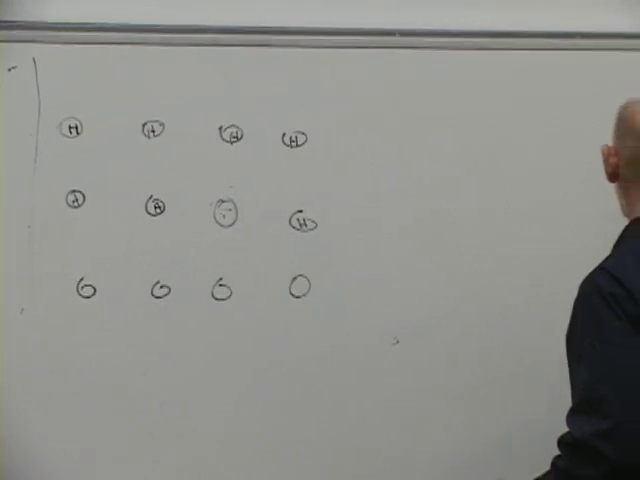
\includegraphics[width=0.9\textwidth]{lecture_06_figure_08.png}
\caption{破線のドメインウォールで分割された表--裏格子。反対の境界条件は、系が二つの縮退した秩序状態の間の界面を含むことを強制する。}
\lectureframe{01:30:35}
\end{figure}

\begin{classroomqa}
\audiencequestion{自発的対称性の破れを通常の明示的対称性の破れと区別するものは何か。
\lecturetimestamp{01:28:36}}
\lecturerresponse{明示的破れでは、局所ハミルトニアンがすでに表と裏に異なるエネルギーを割り当てているので、対称性で関係づけられた基底状態の対は存在しない。自発的破れでは、方程式は対称性を保ち、真空は縮退しており、境界条件または任意に小さな摂動が一方を選ぶ。異なる真空の間を補間するドメインウォールの可能性は、後者の状況の指標である。}
\end{classroomqa}

この模型は意図的に原始的であるが、ヒッグス場に移される本質的な論理を含んでいる：対称な理論、不安定または縮退した真空構造、選ばれた基底状態、そしてその選択によって決まる物理的帰結である。

\section{講義の到達点}

フェルミオン表は標準模型の群を物理的な方向の集合に変える。カラー\(SU(3)\)は赤、緑、青を通って垂直に動く；電荷を持つ弱変換はクォークとレプトンの二重項を通って水平に動く；位相対称性は予備的な\(U(1)\)因子を与える。ゲージボソンの放出はこれらの群変換を相互作用として実現する。

ベータ崩壊の弱さは、例外的に小さな\(g_w\)にではなく、重い媒介粒子に由来する。距離空間では、質量はコンプトン尺度\(\hbar/(m_Wc)\)を超えて伝播関数を遮断する。運動量空間では、
\begin{equation}
  \mathcal A_{\rm weak}
  \sim\frac{g_w^2}{k^2+m_W^2}
  \simeq\frac{g_w^2}{m_W^2}
\end{equation}
核子の運動量において。かつての低エネルギー実験はこの組み合わせをフェルミ定数として測定した。

拡張された教室での議論は、この式が何を意味し何を意味しないかを明らかにする。内部の\(W\)線は仮想でオンシェルではない；エネルギー--運動量は依然として保存される。十分に硬いプローブは実の\(W\)を生成しうるが、そのときには異なる終状態過程を創り出している。衝突生成物は既存の構成要素の文字通りのリストではない。温度は高エネルギー入射粒子の分布を変え、光子は電荷を持つ仮想粒子を通じて相互作用しうるし、ボース統計は力学的な力とは別物である。

最後に、\(SU(2)\)は\(Z\)に関係する欠けている中性ゲージ場を必要とし、表--裏格子は自発的対称性の破れの最初の模型を与える。次の段階は、これら二つの未完成の糸を組み合わせることである：電弱混合とヒッグス機構。